\documentclass[landscape,display]{powersem} %,display
\usepackage{fancybox,marvosym,graphicx,amsmath,amssymb,pifont}
\usepackage[bookmarksopen,colorlinks,urlcolor=red]{hyperref} %,pdfpagemode=FullScreen
%\usepackage[english,vietnam]{babel}
\usepackage[T5,T1]{fontenc}
\DeclareTextSymbolDefault{\acircumflex}{T5}
\DeclareTextSymbolDefault{\DJ}{T5}
\DeclareTextSymbolDefault{\ohorn}{T5}
\DeclareTextSymbolDefault{\uhorn}{T5}

\usepackage{fixseminar}
\usepackage{color}
\usepackage[latin1,utf8]{inputenc}
\usepackage[coloremph,colormath,colorhighlight,lightbackground]{texpower}
\hfuzz=30pt \vfuzz=30pt \setlength{\slidewidth}{25cm}
\setlength{\slideheight}{17.5cm} \slideframe{}
\def\slideitemsep{.5ex plus .3ex minus .2ex}
\renewcommand{\slidetopmargin}{10mm}
\renewcommand{\slidebottommargin}{15mm}
\renewcommand{\slideleftmargin}{5mm}
\renewcommand{\sliderightmargin}{5mm}
\newcommand{\heading}[1]{%
 \begin{center}
  \large\bf
  \shadowbox{{\textcolor{conceptcolor}{#1}}}%
 \end{center}
 \vspace{1ex minus 1ex}}
\backgroundstyle[startcolor=white,
                   endcolor=grey,%firstgradprogression=3,
            rightpanelwidth=-7\semcm,,rightpanelcolor=pagecolor]{hgradient}%
%%%%%%%%%%%%% DATI DEL SEMINARIO IN QUESTIONE %%%%%%%%%%%%

\newpagestyle{327}%
 {\textcolor{codecolor}{\tiny{\textit{Riemann Hypothesis}}} \hspace{\fill}\rightmark
$\pi(x)=\#\{p\leq x\ \textrm{s.t. } p \textrm{ is prime}\}$\hspace{0.3cm}\thepage}
 {\includegraphics[width=4mm]{images/dipmat.pdf}\hspace{\fill}\tiny{\textcolor{codecolor}{\sc Universit\`a Roma Tre}}
 \hspace{\fill}\includegraphics[width=5mm]{images/roma3.pdf}}%%
\pagestyle{327}

\begin{document}
\begin{slide}\pagestyle{empty}
\addtocounter{slide}{-1}
\includegraphics[width=1.6cm]{images/roma3.pdf}\hfill\includegraphics[width=1.9cm]{images/Can_Tho_University.jpg}
\vspace*{-2cm}

\begin{sc}\begin{center}
\small{
{Workshop in Number Theory}\\ \emph{Vietnam}\\ \DJ\d ai H\d oc C\`\acircumflex n Th\ohorn }


September 5, 2015
%\vspace*{1cm}

\vfill
\begin{Large}
\textcolor{underlcolor}{Riemann Hypothesis, History and Ideas}
\end{Large}
\end{center}
\end{sc}


\vfill
\begin{center}\hspace*{2cm}\begin{minipage}{9.5cm}
\textcolor{black}{
 A \textbf{conjecture} 
\textit{(from latin coniect\={u}ra, verb con\={\i}cere, or also 
``interpret, infer, conclude'')}
is a statement or a judgment based on intuition, considered probably true, but not proven.}\medskip

An \textbf{hypothesis} \textit{
(From the ancient greek hypothesis, it is composed with of hypo, ``under'' and thesis, ``position'',
or assumption)} is the premise underlying a reasoning or a proof.
\end{minipage}
\end{center}

\end{slide}

\begin{slide}
\heading{Some conjectures regarding prime numbers: 1/5 }\pause

\textcolor{black}{\textbf{Twin primes Conjecture.}}

\textcolor{red}{There exists infinitely many primes 
$p$ such that $p+2$ is prime}\pause
\vfill

\hspace*{4cm}
\begin{minipage}{7cm}
\textit{for example:} \\
$3$ and $5$,\\ $11$ and $13$,\\ $17$ and $19$,\\ $101$ and $103,$\\ $\vdots$\\
$\vdots$\\ $10^{100}+35737$ and $10^{100}+35739,$ \\ $\vdots$\\
$\vdots\ 3756801695685\cdot2^{666669} \pm 1,$\\ $\vdots$.
\end{minipage}
\end{slide}

\begin{slide}
\heading{Some conjectures regarding prime numbers: 2/5 }\pause

\textcolor{black}{\textbf{Goldbach conjecture}} 

\textcolor{red}{Every even number (except for $2$) can be written as the sum of two primes}\pause
 \includegraphics[width=5cm]{images/Letter_Goldbaxh-Euler.jpg}\pause
\vspace{-5cm}\hspace*{7cm}
\begin{minipage}{4cm}
\textit{for example:} \\
 $42=5+37$,\\ $1000=71+929$,\\ 
$888888=601+888287,$\\ $\vdots$\end{minipage}
\end{slide}

\begin{slide}
\heading{Some conjectures regarding prime numbers: 3/5 }\pause

\textcolor{black}{\textbf{Hardy-Littlewood Conjecture.}} \pause

\textcolor{red}{$\exists$ infinitely many primes $p$ s.t. $p-1$ is a prefect square}\pause
 \includegraphics[width=4cm]{images/hardy.jpg}\pause

\vspace{-3.5cm}
\hspace*{5cm}
\begin{minipage}{7cm}
\textit{for example:} \\
$5=2^2+1$,\\ $17=4^2+1,$\\ $37=6^2+1$,\\ $101=10^2+1$,\\ $\vdots$\\ $677=26^2+1,$\\ $\vdots$\\
$10^{100}+420\cdot10^{50}+42437=(10^{50}+206)^2+1$\\$\vdots$\end{minipage}
\end{slide}

\begin{slide}
\heading{Some conjectures regarding prime numbers: 4/5}\pause

\textcolor{black}{\textbf{Artin Conjecture.}} \pause

\textcolor{red}{ The period of $1/p$ has length $p-1$ for infinitely many primes $p$}\pause


 \includegraphics[width=3cm]{images/EmilArtin.jpg}\pause

\vspace{-4cm}
\hspace*{3.5cm}
\begin{minipage}{8cm}
\textit{for example:} \\
$\frac17=0.\overline{142857}$,\\
\\
$\frac1{17}=0,\overline{0588235294117647}$,\\
\\
$\frac1{19}=0.\overline{052631578947368421},$\\
\\
$\vdots $\\
$\frac1{47}=$\scriptsize{$0.\overline{0212765957446808510638297872340425531914893617} \cdots$}\end{minipage}\bigskip\bigskip\medskip\pause

\begin{scriptsize}
primes with this property: $7, 17, 19, 23, 29, 47, 59, 61, 97, 109, 113, 131, 149, 167, 179, 181, 193,\ldots$
\end{scriptsize}


\end{slide}


\begin{slide}
\heading{Some conjectures regarding prime numbers: 5/5 }

\textcolor{black}{\textbf{Riemann Hypothesis.}\ \ $\zeta(\sigma+it)=0, \sigma\in(0,1)\ \Rightarrow\ \sigma=\frac12$}\pause

\begin{figure}
 \hspace*{1cm}\includegraphics[width=3cm]{images/riemann.jpeg}\\
  {Georg Friedrich Bernhard Riemann}\end{figure}
\vspace*{-0.6cm}\begin{tiny}Birth: 17.09.1826  Breselenz / K\"onigreich Hannover\\
\vspace*{-0.5cm}Death: 20.07.1866  Selasca / Italia
\end{tiny}\pause

\vspace*{-4cm}\hspace*{7cm}
\begin{minipage}{6cm}
\textit{for example:}\\ 
$s_1=\frac12+ 14.135\cdots i,\\ 
s_2=\frac12+21.022\cdots i,\\ 
s_3=\frac12+25.011\cdots i,\\
s_4=\frac12+30.425\cdots i,\\
s_5=\frac12+32.935\cdots i,\\
\vdots\\
s_{126}=\frac12+279.229\cdots i,\\
s_{127}=\frac12+282.455\cdots i,\\
\vdots$\end{minipage}
\end{slide}



\begin{slide}
\heading{The enumerating function of primes}\bigskip\bigskip

\parstepwise{\begin{itemize}
  \item[\textcolor{blue}{\ding{43}}]\step{\textcolor{black}{\textbf{Problem:}} rapidly produce primes $p\approx 10^{150}$};
\bigskip\bigskip
  \item[\textcolor{blue}{\ding{43}}]\step{it is crucial to understand how primes are distributed};
\bigskip\bigskip
  \item[\textcolor{blue}{\ding{43}}]\step{$\displaystyle{\pi(x)=\#\{p\leq x\ \textrm{s.t. } p \textrm{ is prime}\}}$};
\bigskip\bigskip

\item[\textcolor{blue}{\ding{43}}]\step{That is $\pi(x)$ is the number of \emph{prime numbers} up to $x$};
\bigskip\bigskip
\item[\textcolor{blue}{\ding{43}}]\step{\textcolor{green}{Examples:}
$\pi(10)=4$\qquad$\pi(100)=25$\qquad$\pi(1,000)=168$}
\end{itemize}}
\end{slide}

\begin{slide}
\heading{The enumerating function of primes}\bigskip\pause

\centerline{\ovalbox{\begin{Large}
$\displaystyle{\pi(x)=\#\{p\leq x\ \textrm{such that } p \textrm{ is prime}\}}$
            \end{Large}}}\pause\bigskip

\centerline{That is $\pi(x)$ is the number of \emph{prime numbers} up to $x$}\pause
\bigskip
\vfill

\hspace*{5cm}
\begin{minipage}{8cm}
\textit{for example:}\\ 
$\pi(10)=4$,\\
$\pi(100)=25$,\\
$\pi(1,000)=168$\\
$\cdots$\\
$\pi(104729)=10^5$\\
$\cdots$\\
$\pi(10^{24})=18435599767349200867866.$\\
$\cdots$\\
\end{minipage}
\end{slide}

\begin{slide}

\begin{minipage}[l]{7cm}
\begin{scriptsize}
\begin{tabular}{|l|l|}
  \hline
  % after \\: \hline or \cline{col1-col2} \cline{col3-col4} ...
     $x$ & $\pi(x)$\\
\hline
10000 & 1229\\
100000  &   9592\\
1000000  & 78498\\
10000000 & 664579\\
100000000 &    5761455\\
1000000000&   50847534\\
10000000000&  455052511\\
100000000000&     4118054813\\
1000000000000&   37607912018\\
10000000000000&  346065536839\\
100000000000000 & 3204941750802\\
1000000000000000 &29844570422669\\
10000000000000000 &279238341033925\\
100000000000000000 &2623557157654233\\
1000000000000000000 &24739954287740860\\
10000000000000000000 &234057667276344607\\
100000000000000000000 & 2220819602560918840 \\
1000000000000000000000 & 21127269486018731928 \\
10000000000000000000000 & 201467286689315906290\\
\hline
\end{tabular}
\end{scriptsize}
\end{minipage}
\begin{minipage}[r]{4.5cm}
\heading{The plot of $\pi(x)$}
\begin{figure}
\includegraphics[width=4cm]{images/pi100.jpg}
\hspace{1cm} \includegraphics[width=4cm]{images/pi1000.jpg}
 \end{figure}\end{minipage}
\end{slide}            

\begin{slide}
\centerline{\includegraphics[width=11cm]{images/School_of_Athens.jpeg}}\vspace*{-8cm}
\parstepwise{
\step{
      \hspace*{-1mm}\colorbox{white}{\shadowbox{The School of Athens (Raffaello Sanzio)}}
      }
\bigskip\bigskip\bigskip\bigskip\\ %\vspace*{1cm}\hspace*{2cm}
\step{\hspace*{3cm}
      \begin{minipage}{5cm}
                      \shadowbox{\includegraphics[width=3.5cm]{images/Euclid_7.jpeg}}\\
                      \colorbox{white}{\begin{minipage}[c]{4cm}
                               \ \ \ Euclid of Alessandria\vspace*{-2mm}\\
                                 {\tiny Birth: 325 B.C. (approximately)}\vspace*{-2.5mm}\\
                                 {\tiny Death: 265 B.C. (approximately)}
                                \end{minipage}}\\
       \end{minipage}
       }\\ \bigskip\medskip% \bigskip\\
\step{\hspace*{2cm}
      \colorbox{white}{\shadowbox{There exists infinitely many primes: $\pi(x)\rightarrow\infty$ if $x\rightarrow\infty$}}
      }
            }
\end{slide} 


\begin{slide}
\heading{The sieve to count primes}
\bigskip\bigskip

\begin{center}
\includegraphics{images/eratostene.jpg}

220AC  Greeks (Herathostenes from Cirene)
\end{center}   

\end{slide}  

\begin{slide}
\heading{Legendre's Intuition}
\begin{figure}
  \centering \includegraphics[width=3cm]{images/Legendre.jpeg}\\
Adrien-Marie Legendre 1752-1833
 \end{figure}

\heading{$\pi(x)$ is approximately $\displaystyle{\frac{x}{\log x}}$}

\ \hfill\small{$\log x$ is the natural logarithm %(in base $e=2,7182818284590\cdots$) of $x$
}
\end{slide}

% \begin{slide}
% \heading{$\pi(x)$ is approximately $\frac x{\log x}$ }\pause
% 
% \parstepwise{\begin{itemize}
%   \item[\textcolor{blue}{\ding{43}}]\step{\textcolor{black}{\textbf{Che significa $\log x$?}}}\step{\quad is il \emph{logaritmo naturale} of $x$};
% \bigskip  \item[\textcolor{blue}{\ding{43}}]\step{Ricordiamo che il logaritmo in base $a$ of $b$ is quel numero $t$ such that $a^{t}=b$};\\
%  \item[\textcolor{blue}{\ding{43}}]\step{Quindi $t=\log_ab$ significa che $a^t=b$};
% \step{\hspace*{2cm}for esempio $\log_28=3$ perch\`e $2^3=8$}\\
% \step{\hspace*{2cm} and $\log_5625=4$ perch\`e $5^4=625$}.
% 
% \item[\textcolor{blue}{\ding{43}}]\step{Quando la base $a=e=2,7182818284590\cdots$ is the number of Nepero,}\\
% \step{il logaritmo in base $e$ of chiama \emph{logaritmo naturale}};
% 
% \item[\textcolor{blue}{\ding{43}}]\step{\textcolor{green}{perci\`o}
% $\log10=2.30258509299404568401$ perch\`e $e^{2.30258509299404568401}=10$}
% \item[\textcolor{blue}{\ding{43}}]\step{infine $\log x$ is una funzione}
% \end{itemize}}
% 
% \end{slide}

\begin{slide}
% \heading{The function \emph{logaritmo naturale}}
% \begin{figure}
%   \centering \includegraphics[width=4cm]{images/log.jpg} $f(x)=\log x$
%  \end{figure}\pause

\heading{The function $x/\log x$}
\begin{figure}
  \centering \includegraphics[width=10cm]{images/xlog_1.jpg}\\ $f(x)=x/\log x$
 \end{figure}
\end{slide}

\begin{slide}
\heading{$\pi(x)$ is approximately $\frac x{\log x}$ }\pause
that is\vspace*{-2mm}
$\qquad\qquad\displaystyle{
\lim_{x\rightarrow\infty}\frac{\pi(x)}{x/\log x}=1\quad\qquad\text{and it is writtes as}\qquad\quad\pi(x)\sim \frac x{\log x}}$\vspace*{-1mm}\pause
\begin{center}\begin{tiny}
\begin{tabular}{|l|l|l|}
  \hline
  % after \\: \hline or \cline{col1-col2} \cline{col3-col4} ...
     $x$ & $\pi(x)$ & $\frac x{\log x}$\\
\hline
1000   & 168  &   145\\
10000& 1229&  1086   \\
100000&9592&  8686     \\
1000000&   78498& 72382  \\
10000000&  664579& 620420   \\
100000000& 5761455&   5428681\\
1000000000&50847534  & 48254942\\
10000000000&  455052511& 434294482\\
100000000000&     4118054813&3948131654\\
1000000000000&   37607912018&36191206825    \\
10000000000000&  346065536839&334072678387    \\
100000000000000 & 3204941750802&3102103442166   \\
1000000000000000 &29844570422669&28952965460217   \\
10000000000000000 &279238341033925&271434051189532  \\
100000000000000000 &2623557157654233&2554673422960305 \\
1000000000000000000 &24739954287740860&24127471216847324\\
10000000000000000000 &234057667276344607&228576043106974646 \\
100000000000000000000 & 2220819602560918840&2171472409516259138 \\
\hline
\end{tabular}
\end{tiny}\end{center}
\end{slide}

\begin{slide}
\heading{Gau\ss\ Conjecture}
\begin{figure}
  \centering \includegraphics[width=3cm]{images/Gauss_1803.jpeg}\\
Johann Carl Friedrich Gau\ss
(1777 - 1855)
 \end{figure}\pause

\heading{$\pi(x)\sim \displaystyle{\int_{0}^x\frac{du}{\log u}}$}
\end{slide}

% \begin{slide}
% \heading{Cosa significa $\int_{0}^x\frac{du}{\log u}$?}\pause
% 
% \heading{\begin{minipage}{9cm}Cosa is l'integrale of una funzione?\\ (for quelli che non ci sono ancora arrivati)\end{minipage}}\pause
% 
% $$S=\int_a^b f(x)dx$$\pause
% 
% \centerline{\includegraphics[width=4cm]{images/integral.png}}
% 
% \end{slide}


% \begin{slide}
% \heading{The function \emph{Logarithmic Integral}}\pause
% 
% Quindi $f(x)=\int_{0}^x\frac{du}{\log u}$ is una funzione. Ecco il grafico:\pause
% 
% \centerline{\includegraphics[width=5cm]{images/uslog.jpg}\qquad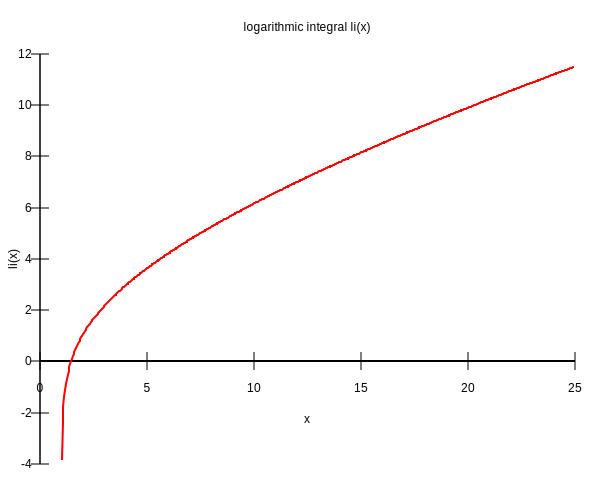
\includegraphics[width=5.5cm]{images/li.jpg}}
% 
% $1/\log x$\hfill $\operatorname{li}(x)$
% \end{slide}

\begin{slide}
\heading{The function \emph{Logarithmic Integral}}\pause

We set $\operatorname{li}(x)=\int_{0}^x\frac{du}{\log u}$, the function \emph{Logarithmic Integral}. Here is the plot:\pause

\begin{figure}
  \centering \includegraphics[width=8cm]{images/li_1.jpg}\\ $\operatorname{li}(x)$
 \end{figure}

\end{slide}

\begin{slide}
\heading{More recent photo of Gau\ss}
\begin{center}\begin{figure}
  \includegraphics[width=6cm]{images/Gauss_banknote.jpeg}\bigskip\bigskip\vspace{-1.3mm} \\
Johann Carl Friedrich Gau\ss (1777 - 1855)
 \end{figure}\end{center}

\heading{$\pi(x)\sim\operatorname{li}(x):=\displaystyle{\int_{0}^x\frac{du}{\log u}}$}
\end{slide}

\begin{slide}
\heading{The function "logarithmic integral" of Gau\ss}
$$\operatorname{li}(x)=\int_{0}^x\frac{du}{\log u}$$

\begin{center}\begin{tiny}
\begin{tabular}{|l|l|l|l|}
  \hline
  % after \\: \hline or \cline{col1-col2} \cline{col3-col4} ...
     $x$ & $\pi(x)$ & $\operatorname{li}(x)$ & $\frac x{\log x}$\\
\hline
1000                 & 168               &   178     &   145\\
10000                & 1229              &  1246     &  1086   \\
100000               &9592               &  9630     &  8686     \\
1000000              &   78498           & 78628     & 72382  \\
10000000             &  664579           &664918     & 620420   \\
100000000            & 5761455           &   5762209 &   5428681\\
1000000000           &50847534           &50849235   & 48254942\\
10000000000          &  455052511        & 455055614 & 434294482\\
100000000000         &     4118054813    &4118066401&3948131654\\
1000000000000        &   37607912018     &37607950281&36191206825    \\
10000000000000       &  346065536839     &346065645810&334072678387    \\
100000000000000      & 3204941750802     &3204942065692&3102103442166   \\
1000000000000000     &29844570422669     &29844571475288&28952965460217   \\
10000000000000000    &279238341033925    &279238344248557&271434051189532  \\
100000000000000000   &2623557157654233   &2623557165610822&2554673422960305 \\
1000000000000000000  &24739954287740860  &24739954309690415&24127471216847324\\
10000000000000000000 &234057667276344607 &234057667376222382&228576043106974646 \\
100000000000000000000&2220819602560918840&2220819602783663484&2171472409516259138 \\
\hline
\end{tabular}
\end{tiny}  \end{center}
\end{slide}

\begin{slide}
\heading{The function \emph{$\operatorname{li}(x)$} vs $\frac{x}{\log x}$}\pause


\begin{figure}
  \centering \includegraphics[width=8cm]{images/xlogli.jpeg}
 \end{figure}\pause

\centerline{\ovalbox{$\operatorname{li}(x)=\displaystyle{\frac x{\log x}}+\int_{0}^x\frac{dt}{\log^2t}\sim\displaystyle{\frac x{\log x}}$}}

\hfill via integration by parts
\end{slide}


\begin{slide}
\heading{Chebyshev Contribution}

\begin{tabular}{|cc|}
\hline
\begin{minipage}[c]{5cm}
\includegraphics[width=4cm]{images/Chebyshev1.jpg}\\
Pafnuty Lvovich Chebyshev\\
1821 - 1894
\end{minipage}&
\begin{minipage}[c]{5.5cm}
\begin{sc}Chebyshev's Theorems\end{sc}
\begin{itemize}
\item $\frac78 \leq \frac{\displaystyle{\pi(x)}}{\displaystyle{\frac x{\log x}}}\leq \frac98$
\item $\displaystyle{\liminf_{x\rightarrow\infty}}\frac{\pi(x)}{x/\log x}\leq1$
\item $\displaystyle{\limsup_{x\rightarrow\infty}}\frac{\pi(x)}{x/\log x}\geq1$
\item $\forall n$, $\exists p$, $n<p<2n$\\ (Bertrand Postulate)
\end{itemize}
\end{minipage}\\
\hline
\end{tabular}

\end{slide}



\begin{slide}
\heading{Great problem of the end of 800:}\bigskip\pause

\parstepwise{\begin{itemize}
  \item[\textcolor{blue}{\ding{43}}]\step{Prove the Legendre -- Gau\ss\ \emph{Conjecture}\ }
\restep{{{$\displaystyle{\pi(x)\sim\frac{x}{\log x}}$ if $x\rightarrow\infty$}}}
  \item[\textcolor{blue}{\ding{43}}]\step{that is:\ \ }
\restep{{{$\displaystyle{\left|\frac{\pi(x)}{\frac{x}{\log x}}-1\right|\rightarrow0}$ if $x\rightarrow\infty$}}}\bigskip
  \item[\textcolor{blue}{\ding{43}}]\step{that is:\ \ }
\restep{{{$\displaystyle{\left|\pi(x)-\frac{x}{\log x}\right|}$ is ``much smaller'' than
$\displaystyle{\frac{x}{\log x}}$ if  $x\rightarrow\infty$}}}
 \item[\textcolor{blue}{\ding{43}}]\step{that is:\ \ }
\restep{$\displaystyle{\left|\pi(x)-\frac{x}{\log x}\right|=o\left(\frac{x}{\log x}\right)}$ if  $x\rightarrow\infty$}
  \item[\textcolor{blue}{\ding{43}}]\step{that is (to say it at the Gau\ss\ way):}
\restep{{{$\displaystyle{|\pi(x)-\operatorname{li}(x)|}=o\left(\operatorname{li}(x)\right)$ if  $x\rightarrow\infty$}}}
\end{itemize}}
\pause
%\item[\textcolor{blue}{\ding{43}}]\step{molto lavoro:}
%\restep{\emph{Gau\ss, Riemann, Chebyshev, von Mangoldt, Hadamard, de la Vall\'ee Poussin,...}}

This statement is historically referred to as \emph{The Prime Number Theorem.}

\end{slide}




\begin{slide}
\heading{Riemann's paper 1859}
\vspace{-0.5cm}

\begin{tabular}{|cc|}
\hline
\begin{minipage}[c]{5cm}
\includegraphics[width=4cm]{images/riemann1859_1.pdf}\vspace{-2mm}\\
{\tiny{(Ueber die Anzahl der Primzahlen unter
einer gegebenen Gr\"osse.)
Monatsberichte der Berliner Akademie,1859}}
\end{minipage}&
\begin{minipage}[c]{5.5cm}
\textcolor{red}{\begin{sc}Riemann Hypothesis:\end{sc}}
\begin{large}$$|\pi(x)-\operatorname{li}(x)|\ll\sqrt{x}\log x$$\end{large}
\\
\begin{sc}Revolutionary Idea:\end{sc}\\
Use the function:
\begin{small}$$\zeta(s)=\sum_{n=1}^\infty\frac1{n^s}$$\end{small}
and \emph{complex analysis}.\\
%(i.e. $s\in\mathbb C$)\\
\end{minipage}\\
\hline
\end{tabular}
\end{slide}

\begin{slide}
\heading{Summery:}\bigskip\bigskip\pause

\parstepwise{\begin{itemize}
  \item[\textcolor{blue}{\ding{43}}]\step{Riemann Hypothesis (1859)} 
  \restep{{\ovalbox{$|\pi(x)-\operatorname{li}(x)|\ll\sqrt{x}\log x$}}}\smallskip
\item[\textcolor{blue}{\ding{43}}]\step{\textcolor{black}{Riemann} doe not complete the proof of the \emph{Prime Number Theorem}
}\\
\restep{but he suggests the right path.}\smallskip
    \item[\textcolor{blue}{\ding{43}}]\step{The idea to use the $\zeta$ function as a complex variable function}\smallskip
\item[\textcolor{blue}{\ding{43}}]\step{\textcolor{black}{Hadamard} and \textcolor{black}{de la Vall\'ee Poussin (1897)} 
add the missing piece to}
\restep{\textcolor{black}{Riemann}'s program and prove the \emph{Prime Number Theorem}}
\restep{\centerline{\ovalbox{$|\pi(x)-\operatorname{li}(x)|\ll x\exp\left(-\sqrt{\log x}\right).$}}}\smallskip
\item[\textcolor{blue}{\ding{43}}]\step{The use of $\zeta$ to study primes had already been suggested by \textcolor{black}{Euler}!!}
\item[\textcolor{blue}{\ding{43}}]\step{Schoenfeld (1976),  Riemann Hypothesis is equivalent to}\\
\restep{\centerline{\ovalbox{$|\pi(x) - \operatorname{li}(x)| < \frac{1}{8\pi} \sqrt{x} \log(x)$ if $x\ge2657$}}}
\end{itemize}}

     
\end{slide}




\begin{slide}
\heading{Prime Number Theorem finally proven (1896)}

\begin{tabular}{|cc|}
\hline
\begin{minipage}[c]{5cm}
\includegraphics[width=4cm]{images/Hadamard.jpeg}\\
{\tiny{Jacques Salomon Hadamard 1865 - 1963}}
\end{minipage}&
\begin{minipage}[c]{5cm}
\includegraphics[width=4cm]{images/Vallee_Poussin_2.jpeg}\vspace{-2.9mm}\\
{\tiny{Charles Jean Gustave Nicolas\vspace{-2.9mm}\\ Baron de la Vall\'ee
Poussin 1866 - 1962}}
\end{minipage}\\
\hline
\end{tabular}\bigskip\pause
\hspace*{3cm}\ovalbox{$\displaystyle{|\pi(x)-\operatorname{li}(x)|\ll x\exp(-a\sqrt{\log x})\quad \exists a>0}$}
\end{slide}

\begin{slide}
\heading{Euler Contribution}
\begin{center}\begin{figure}
  \includegraphics[width=4cm]{images/Euler_9.jpeg}\\ 
Leonhard Euler (1707 - 1783)
 \end{figure}\end{center}

\heading{$\displaystyle{\zeta(s)=\sum_{n=1}^\infty\frac1{n^s}}$ is related to prime numbers}
\end{slide}

\begin{slide}\addtocounter{slide}{-1}
\heading{Euler Contribution}
\begin{center}\begin{figure}
  \includegraphics[width=6cm]{images/euler1.jpg}\bigskip\bigskip\bigskip\bigskip\vspace{1mm}\\
Leonhard Euler (1707 - 1783)
 \end{figure}\end{center}

\heading{$\displaystyle{\zeta(s)=\sum_{n=1}^\infty\frac1{n^s}}=\prod_{p\text{\ prime}}\left(1-\frac1{p^s}\right)^{-1}$}
\end{slide}

\begin{slide}
\heading{The beautiful formula of Riemann}\pause

\ \ \ \ \ \ \ \ \ \ \Ovalbox{$\zeta(s)=\displaystyle\sum_{n=1}^\infty\frac1{n^s}=\pi^{\frac s2}\frac{\displaystyle{\frac1{s(s-1)}+\int_1^\infty\left(x^{\frac s2-1}+
x^{-\frac{s+1}2}\right)\left(\sum_{n=1}^\infty e^{-n^2\pi x}\right)dx}}
{\displaystyle\int_0^\infty e^{-u}u^{\frac s2-1}\frac{du}u}
$}\pause\vspace*{-0.2cm}
\heading{Exercise}
Show that, if $\sigma,t\in\mathbb R$ are such that
$$\begin{cases}\displaystyle{\int_1^\infty \frac{\{x\}}{x^{\sigma+1}}\cos(t\log x)dx=\frac{\sigma}{(\sigma-1)^2+t^2}}\\\\\displaystyle{\int_1^\infty \frac{\{x\}}{x^{\sigma+1}}\sin(t\log x)dx=\frac{t}{(\sigma-1)^2+t^2}}\end{cases}$$
Then $\sigma=\frac12$.\hfill\qquad\qquad\tiny{ (Here $\{x\}$ is the \emph{fractional part} of $x\in\mathbb R$.)}\end{slide}

\begin{slide}\pageTransitionWipe{30}
\heading{Explicit distribution of prime numbers}\pause

%$$\pi(x)=\#\{p\leq x\ \textrm{s.t. } p \textrm{ is prime}\}$$\pause


\begin{center}
\begin{tabular}{|c|}\hline
\textbf{\textcolor{red}{Theorem.}} (Rosser - Schoenfeld) if $x\geq 67$\\
 $\displaystyle{\frac{x}{\log x-1/2}< \pi(x)< \frac{x}{\log x-3/2}}$\\
\hline\end{tabular}
\end{center}\pause

Hence

 $\frac{10^{100}}{\log(10^{100})-1/2}<\pi(10^{100})< \frac{10^{100}}{\log(10^{100})-3/2}$\pause

\begin{tiny}
$$\hspace*{-0.5cm}43523959267026440185153109567281075805591550920049791753399377550746551916373349269826109730287059.61758148$$
\end{tiny}\vspace*{-5mm}
$$< \pi(10^{100})< $$
\begin{tiny}
$$\hspace*{-0.5cm}43714220863853254827942128416877119789366015267226917261629640806806895897149988858712131777940942.89031$$
\end{tiny}

\end{slide}

\begin{slide}
\heading{The five conjectures today -- any News?}\pause

\textcolor{blue}{\ding{43}}
\textcolor{black}{\textbf{twin primes.}} {There existes infinitely many primes 
$p$ such that $p+2$ is prime}; that is\pause
\centerline{\ovalbox{$\displaystyle{\liminf_{n\rightarrow\infty}\left(p_{n+1}-p_n\right)=2}$}}
\ \ \hfill \small{$p_1=2,\ p_2=3, p_3=5,\cdots,p_n$ is the $n$--th prime}\pause

\textcolor{blue}{\ding{43}} {Enrico Bombieri and Harald Davenport in 1966};\pause
\centerline{\ovalbox{$\displaystyle{\liminf_{n\rightarrow\infty}\frac{p_{n+1}-p_n}{\log p_n}< 0.46\cdots}$}}
\ \ \  \hfill \small{in other words, for infinitely many $n$, $(p_{n+1}-p_n)<0,46\cdots \log p_n$}\pause

\textcolor{red}{\ding{44}} Daniel Goldston, J\'anos Pintz and Cem Yildirim in 2005;\pause
\centerline{\ovalbox{$\displaystyle{\liminf_{n\rightarrow\infty}\frac{p_{n+1}-p_n}{\sqrt{\log p_n}\log\log p_n}=0}$}}

\textcolor{green}{\ding{44}} Yitang Zhang on May 14, 2013;\pause
\centerline{\ovalbox{$\displaystyle{\liminf_{n\rightarrow\infty}\left(p_{n+1}-p_n\right)\le 7\cdot 10^7}$}}

\end{slide}


\begin{slide}
 \heading{Zhang Contribution}
\begin{center}\begin{figure}
  \includegraphics[width=3cm]{images/zhang.jpeg}\\ 
Yitang Zhang\\ (\texttt{http://en.wikipedia.org/wiki/Yitang\_Zhang})
 \end{figure}\end{center}

\heading{May 14, 2013: $\displaystyle{\liminf_{n\rightarrow\infty}\left(p_{n+1}-p_n\right)\le 70.000.000}$}
\end{slide}

\begin{slide}
 \heading{The race of the summer 2013 started on May 14,}

\centerline{\scriptsize{\texttt{http://michaelnielsen.org/polymath1/index.php?title=Timeline\_of\_prime\_gap\_bounds}}}\pause

\heading{May 14, 2013: $\displaystyle{\liminf_{n\rightarrow\infty}\left(p_{n+1}-p_n\right)\le 70.000.000}$}

\begin{center}\begin{figure}
  \includegraphics[width=13cm]{images/Schermata1.png}
 \end{figure}\end{center}
\end{slide}

\begin{slide}
 \heading{The race of the summer 2013 started on May 14,}

\centerline{\scriptsize{\texttt{http://michaelnielsen.org/polymath1/index.php?title=Timeline\_of\_prime\_gap\_bounds}}}\pause

\heading{June 15, 2013: $\displaystyle{\liminf_{n\rightarrow\infty}\left(p_{n+1}-p_n\right)\le 60.764}$}

\begin{center}\begin{figure}
  \includegraphics[width=13cm]{images/Schermata2.png}
 \end{figure}\end{center}
\end{slide}

\begin{slide}
 \heading{The race of the summer 2013 started on May 14,}

\centerline{\scriptsize{\texttt{http://michaelnielsen.org/polymath1/index.php?title=Timeline\_of\_prime\_gap\_bounds}}}\pause

\heading{July 27, 2013: $\displaystyle{\liminf_{n\rightarrow\infty}\left(p_{n+1}-p_n\right)\le 4.680}$}

\begin{center}\begin{figure}
  \includegraphics[width=13cm]{images/Schermata3.png}
 \end{figure}\end{center}
\end{slide}

\begin{slide}
 \heading{The race of the summer 2013 started on May 14,}

\centerline{\scriptsize{\texttt{http://michaelnielsen.org/polymath1/index.php?title=Timeline\_of\_prime\_gap\_bounds}}}\pause

\heading{January 6, 2014: $\displaystyle{\liminf_{n\rightarrow\infty}\left(p_{n+1}-p_n\right)\le 270}$}

\begin{center}\begin{figure}
  \includegraphics[width=13cm]{images/Schermata4.png}
 \end{figure}\end{center}
\end{slide}

\begin{slide}
 \heading{The race of the summer 2013 started on May 14,}

\centerline{\scriptsize{\texttt{http://michaelnielsen.org/polymath1/index.php?title=Bounded\_gaps\_between\_primes}}}\pause

\heading{Race to the solution of a more general problem}\pause

$H_m=$ least integer s.t. among $n,n+1,\cdots,n+H_m$ there are $m$ consecutive primes\pause

\begin{center}\begin{figure}
  \includegraphics[width=12cm]{images/Schermata5.png}
 \end{figure}\end{center}
\end{slide}

\begin{slide}
 \heading{Polymath8 and Terry Tao}

\begin{center}\begin{figure}
  \includegraphics[width=10cm]{images/gr_terencetao_wideweb__470x313,0.jpg}
 \end{figure}\end{center}



\end{slide}


\begin{slide}
\heading{The five conjectures today -- any News?}\pause

\textcolor{blue}{\ding{43}}\textcolor{black}{\textbf{Goldbach conjecture}} 

\textcolor{red}{Every even number (except for $2$) can be written as the sum of two primes}\pause
 \includegraphics[width=3cm]{images/petros_en.jpg}\pause
\vspace{-2cm}\hspace*{4cm}
\begin{minipage}{7cm}
\textsc{Equivalent formulation:}\\
\\
every integer greater than $5$ \\
can be written as the sum of three primes\end{minipage}

\end{slide}

\begin{slide}
 \heading{From Vinogradov to Helfgott}

 \includegraphics[width=6cm]{images/helfgott.jpg}\\ \ \ \ \ \ \ \ \ Harald Helfgott\pause
\vspace{-4cm}\hspace*{6cm}
\begin{minipage}{5cm}
\begin{itemize}
 \item (Vinogradov -- 1937) every odd integer greater than  $3^{3^{15}}$  is the sum of three primes
 \item (Helfgott -- 2013) every odd integer greater than 5 is the sum of three primes
\end{itemize}
\end{minipage}
\end{slide}

\begin{slide}
 \heading{Hooley's Contribution}

\textcolor{black}{\textbf{Riemann Hypothesis implies Artin Conjecture.}} \pause

\textcolor{red}{ The period of $1/p$ has length $p-1$ for infinitely many primes $p$}\pause

\begin{minipage}{8cm}
\textit{for example:} \\
$\frac17=0.\overline{142857}$,\\
\\
$\frac1{17}=0,\overline{0588235294117647}$,\\
\\
$\frac1{19}=0.\overline{052631578947368421},$\\
\\
$\vdots $\\
$\frac1{47}=$\scriptsize{$0.\overline{0212765957446808510638297872340425531914893617} \cdots$}\end{minipage}\medskip\pause

\begin{scriptsize}
Primes with this property: $7, 17, 19, 23, 29, 47, 59, 61, 97, 109, 113, 131, 149, 167, 179, 181, 193,\ldots$
\end{scriptsize}
\end{slide}
\end{document}

\begin{slide}
 \heading{News on the other three problems}

\parstepwise{\begin{itemize}
 
\item[\textcolor{blue}{\ding{43}}]\step{\textcolor{black}{\textbf{Hardy-Littlewood.}} $\exists$ infinitely many
primes $p$ s.t. $p-1$ is a prefect square};%\\
%\step{\hspace*{1cm}\textit{ for example: $5=2^2+1$, $37=6^2+1$, $677=26^2+1...$}}
\item[\textcolor{blue}{\ding{43}}]\step{\textcolor{black}{\textbf{Artin}} The period of $1/p$ has length $p-1$
for infinitely many primes $p$};%\\
%\step{\textit{ for example: $\frac17=0.\overline{142857}$, $1/19=0.\overline{052631578947368421}$,}}\\
%\step{\hspace*{1cm} $1/47=0.\overline{0212765957446808510638297872340425531914893617}
%...$}
\item[\textcolor{blue}{\ding{43}}]\step{\textcolor{black}{\textbf{Riemann Hypothesis.}}}
\end{itemize}}
\end{slide}





